\section{Dataset Analysis}
\label{sec:dataset}

Multiple iterations of the recording process were run to find the best possible setup, which reduces the light interference as much as possible and which offers the best results with the resources at hand. The camera setup that is used by SilverFit was reproduced. At SilverFit the camera is mounted at $175cm$ above the floor. The camera that is used has an accelerometer which was used to adjust the camera angle relative to the ground. The camera is angled downward at a $70^\circ$ angle. To record the dataset an Intel Realsense L515 camera was used. Additionally, for the preliminary analysis of errors an Orbbec Astra+ and a Microsoft Kinect v2 were used.

\subsection{Distribution of Errors}

An important aspect of the dataset is the structure and distribution of data and their labels. In total, all 13 exercises mentioned in section \ref{sec:exercises} were recorded twice. Each recording session consists of exactly 300 frames.

When multiple persons are detected one person might be incorrectly detected in the background. While analysing the data the person that is not labelled as faulty is selected whenever possible. If a person is labelled as faulty each joint is marked as in an unrealistic position.

An important factor in how well a model can be trained on data is the balance of the dataset. In this case, the dataset is balanced by the error labels. 

\subsubsection{Full Body Error Distribution}

In Figure \ref{fig:fb_pie} the error distribution of the Full body problem set can be seen. It can be observed that the distribution of errors is reasonably equal with a difference of $10\%$. 

\begin{figure}[ht]
  \centering
  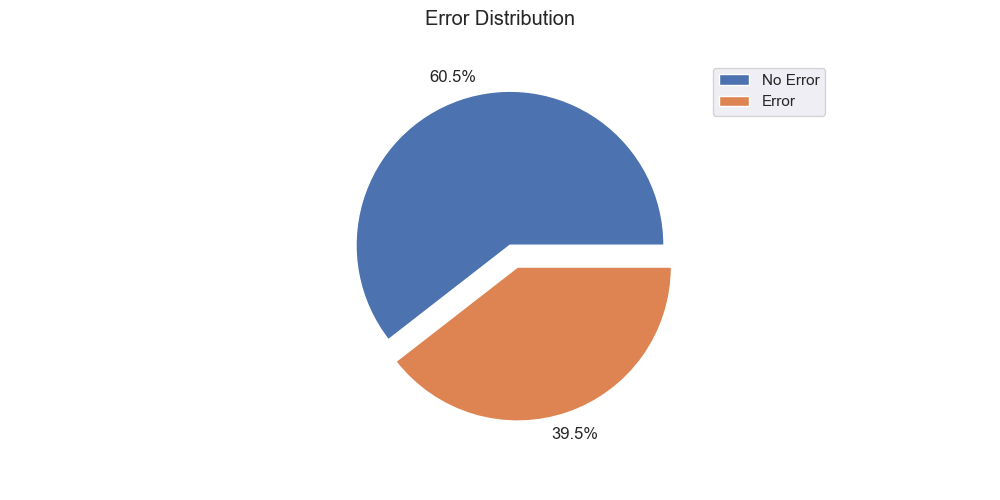
\includegraphics[width=0.4\textwidth]{figures/Data/dist_full_body/Error_Distribution_by_Body_Half.png}
  \caption[Error Distribution of the Full Body]{The distribution of Errors of the full body problem set.}
  \label{fig:fb_pie}
\end{figure}

\subsubsection{Half Body Error Distribution}

Figure \ref{fig:hb_pie} shows a discrepancy between the error distribution of the lower body ($65.4\%$ Errors) and the upper body ($32.4\%$ Errors). The upper body is generally more stable and less error-prone than the lower body.

\begin{figure}[ht]
  \centering
  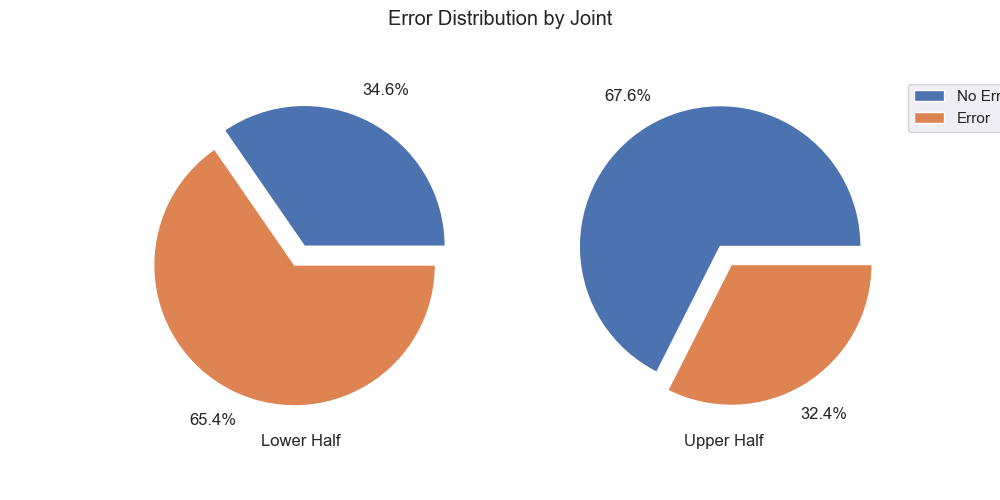
\includegraphics[width=0.6\textwidth]{figures/Data/dist_half_body/Error_Distribution_by_Joint.png}
  \caption[Error Distribution by Body Half]{The distribution of Errors of the half body problem set.}
  \label{fig:hb_pie}
\end{figure}

\subsubsection{Body part Error Distribution}

The error distribution of each body part is shown in figure \ref{fig:lb_pie}. It can be observed that the errors of the body parts are individually very unbalanced. The left arm is the most error-prone body part with $24.1\%$ of the joints being faulty. The torso is the least error-prone body part with $10.3\%$ of the joints being faulty. This again underlines the assumption that the upper body is more stable than the lower body.

\begin{figure}[ht]
  \centering
  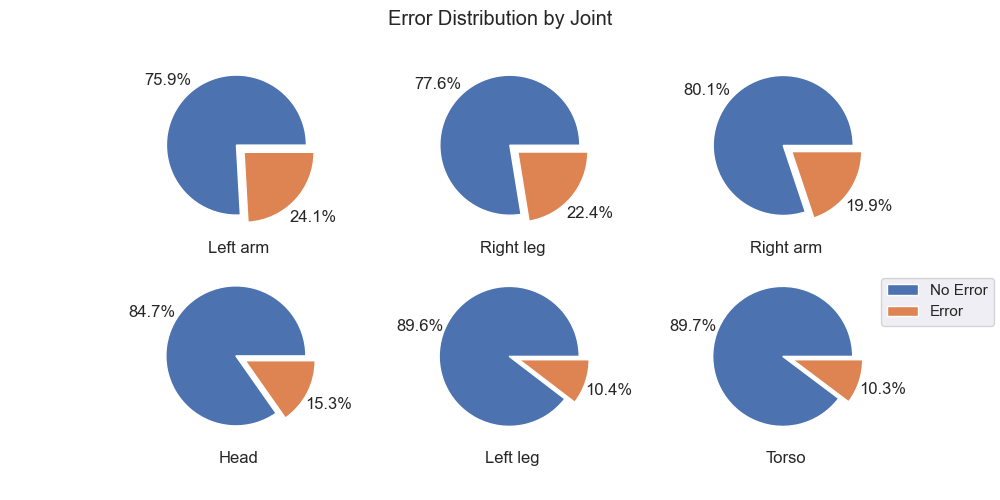
\includegraphics[width=0.8\textwidth]{figures/Data/dist_limbs/Error_Distribution_by_Joint.png}
  \caption[Error Distribution by Body part]{The distribution of errors of the body part problem set.}
  \label{fig:lb_pie}
\end{figure}

\subsubsection{Joint Error Distribution}

Figure \ref{fig:jt_pie} shows that the major part of the errors that occur are errors with the label 2, i.e. the joint is detected in the wrong place. The second most common error is label 1, i.e. the joint is not detected at all. The least common error is label 3, i.e. the joint is detected in the approximate position of where another joint should be.

\begin{figure}[ht]
  \centering
  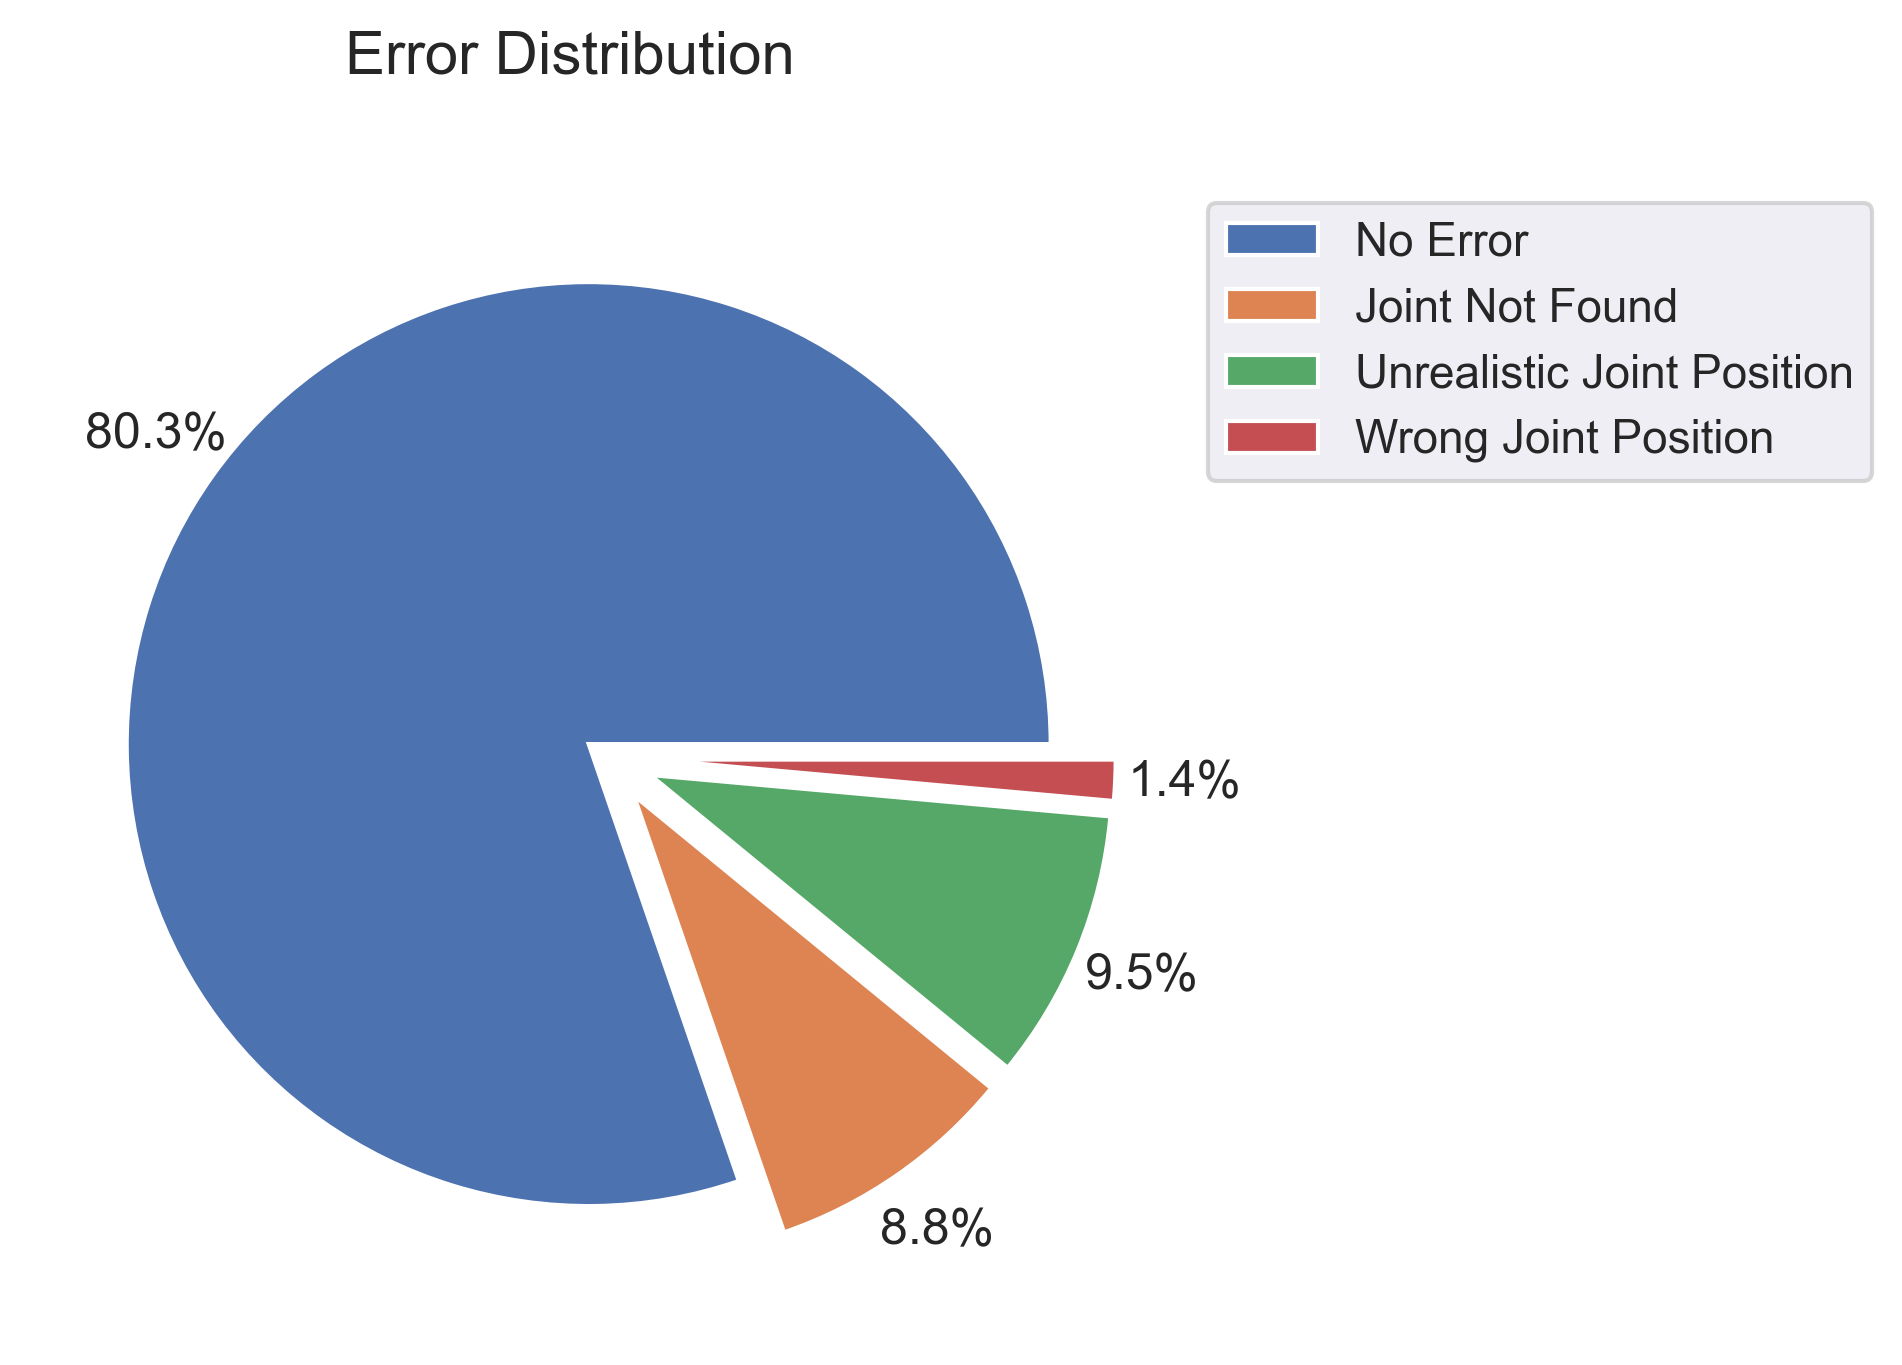
\includegraphics[width=0.4\textwidth]{figures/Data/dist_joints/Error_Distribution.png}
  \caption[Error Distribution for each error class]{The distribution of each error class.}
  \label{fig:jt_pie}
\end{figure}

